\chapter{Metodologia}

\todo[inline]{O capítulo todo é um resumo do CRISP-DM 1.0... fico dando \cite em todo parágrafo?}

\section{Processo CRISP-DM 1.0}

% Por que seguir um processo?
\todo[inline]{Por que um processo?}

% Reproducibilidade/padronização/etc
\cite{ML_know} \cite{balance-anarchy} \cite{ML_debt} \cite{replicability}

% Por que CRISP-DM?
\todo[inline]{Por que CRISP-DM?}
\cite{CRISP-DM-KDD-SEMMA}

% História do CRISP-DM
%% p. 1-2
\todo[inline]{História do CRISP-DM}
CRISP-DM(CRoss-Industry Standard Process for Data Mining) é um processo de aplicação de Mineração de Dados, desenvolvido pelo CRISP-DM Special Interest Group e publicado em 2000. Foi concebido em 1996 por três empresas que utilizavam Mineração de Dados: DaimlerChrysler(à época Daimler-Benz), SPSS(à época ISL) e NCR; motivadas pela incerteza com relação à qualidade de seus trabalhos, pelo questionamento de se toda nova empresa que quiser aplicar Mineração de Dados terá que passar pelo aprendizado que passaram, baseado em tentativa e erro, e como garantir, para seus clientes, que Mineração de Dados era uma área suficientemente madura para ser incorporada a seus processos de negócio. Em 1999 foi publicado um draft do CRISP-DM versão 1.0, sendo aplicado pela DaimlerChrysler, SPSS e NCR a vários tipos de aplicações, indústrias e problemas de negócio, sendo considerado, então, validado suficientemente para ser publicado e distribuído\cite{CRISP-DM}.
\todo[inline]{E hoje em dia?}

% Overview do CRISP-DM
%% p. 6
\todo[inline]{figura com diagrama}
\todo[inline]{Overview}
CRISP-DM segue uma estrutura hierárquica, composta de quatro níveis de abstração(do mais genérico ao mais específico):\todo{traduzir ou não?} fase, tarefa genérica, tarefa especializada e instância de processo. Os dois primeiros níveis, fase e tarefa genérico, foram modelados a fim de serem genéricos o suficiente para atenderem às todas aplicações de Mineração de Dados; completos, abrangendo todo o processo de Mineração de Dados; e estáveis, sendo aplicáveis tanto para as técnicas de Mineração de Dados existentes, quanto às que venham a ser desenvolvidas. O terceiro nível, tarefa especializada, é composto pelas tarefas a serem executadas em situações específicas para alcançar os objetivos das tarefas genéricas. Exemplificando, seja a tarefa genérica Limpar dados: a ela relacionadas estão as tarefas especializadas Limpar dados numéricos e Limpar dados categóricos. O quarto nível, instância de processo, é composto pelos registros de ações, decisões e resultados de uma execução do processo.\cite{CRISP-DM}

% Sobre não ser linear, mas interativo incremental
Apesar de a representação do processo sugerir que ele é composto por uma sequência fixa de fases, na prática as tarefas podem ser executadas seguindo outras ordens: é o caso de, por exemplo, na tarefa Avaliação do modelo ser verificado que são necessários mais dados, a serem adquiridos através de tarefas que, de acordo com o diagrama, já foram executadas.

% Mapeamento modelo -> instância
%% p. 7-8
Para o mapeamento do modelo em uma instância do processo, a especificação do CRISP-DM 1.0 identifica como relevantes quatro dimensões do contexto de Mineração de Dados: domínio de aplicação, tipo de problema de Mineração de Dados, aspectos técnicos e ferramentas e técnicas. Os valores dessas dimensões são utilizados nas decisões sobre que tarefas específicas podem ou devem ser executadas.

O processo de mapeamento do CRISP-DM a uma instância do processo é, de acordo com o CRISP-DM 1.0, composto pelas etapas:
\begin{enumerate}
\item Analisar o contexto, identificando os valores para as dimensões domínio de aplicação, tipo de problema de Mineração de Dados, aspectos técnicos e ferramentas e técnicas
\item Remover do modelo CRISP-DM os detalhes não aplicáveis ao contexto analisado
\item Adicionar detalhes específicos do contexto analisado
\item Especializar(ou instanciar) elementos genéricos do modelo de acordo com características concretas do contexto
\item Possivelmente renomear elementos genéricos do modelo a fim de tornar mais explícito seu significado, de acordo com o contexto
\end{enumerate}

\todo[inline]{tabela com exemplos de valores para as dimensões -> p.7}

\todo[inline]{figura com representação do processo}
\begin{figure}[H]
	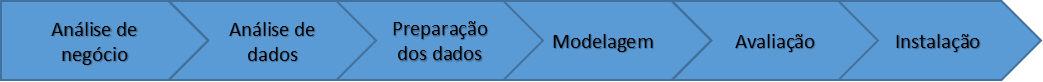
\includegraphics[scale=0.8]{img/CRISP-DM-main.png}
	\caption{Fases do CRISP-DM}
	\label{img:CRISP-DM-diagram}
\end{figure}

% Overview das fases 
%% p. 10-11
A seguir segue uma descrição breve de cada uma das fases:

\begin{enumerate}

\item \textbf{Análise do negócio}:
O objetivo desta fase é entender os requisitos e objetivos do projeto sob uma perspectiva de negócio, traduzí-los para requisitos e objetivos sob uma perspectiva de Mineração de Dados e então traçar um plano preliminar para alcançá-los.

\item \textbf{Análise dos dados}:
Esta fase inicia com uma coleta inicial de dados e segue para o estudo dos dados a fim de identificar problemas de qualidade, obter insights e detectar possíveis subconjuntos de dados que permitam desenvolver hipóteses sobre informações que não estejam presentes.

\item \textbf{Preparação dos dados}:
Esta fase é composta por atividades necessárias para gerar, a partir dos dados inicialmente coletados, um conjunto de dados a ser utilizado pelas ferramentas de modelagem. Inclui atividades como seleção de tabelas, registros, atributos, transformações e limpeza de dados.

\item \textbf{Modelagem}:
Nesta fase são aplicadas técnicas de modelagem e os modelos desenvolvidos são otimizados. Normalmente aplicam-se ao problema mais de uma técnicas de modelagem. Como algumas técnicas de modelagem podem exigir que os dados estejam em dado formato, pode ser necessário voltar para a fase Preparação dos dados.

\item \textbf{Avaliação}:
Esta fase é iniciada quando já foi desenvolvido um modelo com alta qualidade, do ponto de vista da Mineração de Dados. Nela são avaliados a adequação do modelo como ferramenta para alcançar o objetivo de negócio que motivou o projeto e a qualidade da instância do processo. Ela termina com a decisão pela utilização ou não dos resultados obtidos.

\item \textbf{Instalação}:\todo{qual a tradução para deployment?}
Após o desenvolvimento de um modelo, faz-se necessário que ele seja disponibilizado para os usuários finais, seja na forma de relatórios, seja na forma de sistemas de apoio à tomada de decisão, para que seja efetivamente utilizado, auxiliando no alcance dos objetivos de negócio que motivaram a criação do projeto.

\end{enumerate}

\subsection*{Análise do negócio}

\begin{figure}[H]
	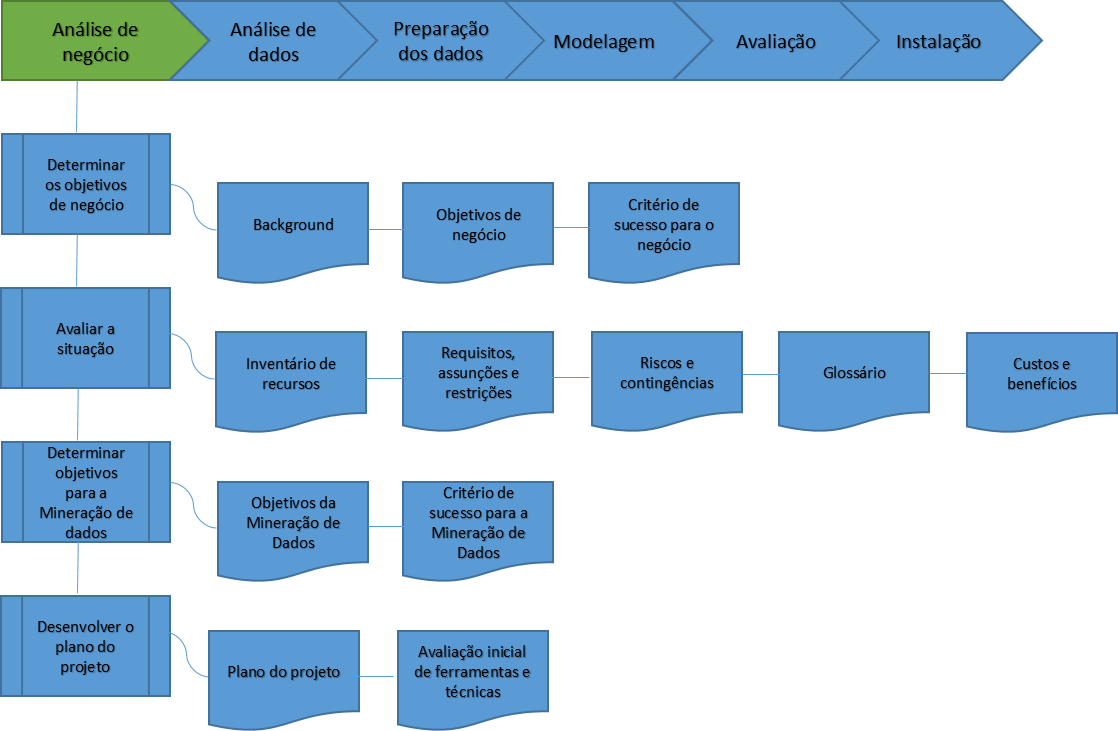
\includegraphics[scale=0.8]{img/CRISP-DM-Analise-de-negocio.png}
	\caption{Detalhamento da fase Análise de negócio}
	\label{img:CRISP-DM-analise-de-negocio}
\end{figure}


\subsection*{Análise dos dados}
\subsection*{Preparação dos dados}
\subsection*{Modelagem}
\subsection*{Avaliação}
\subsection*{Instalação}

\section{Ferramentas utilizadas}